Эта часть сделана Александром Шабалиным

\subsection{Описание выбранного метода}\label{subsec:описание-выбранного-метода}
Для детектирования лиц была использована архитектура нейронной сети RetinaFace.
Она состоит из двух частей: основной модели и пирамиды признаков.
Основная модель - это сверточная нейронная сеть, предназначенная для выявления признаков из изображения.
В качестве основной модели может выступать MobileNet, VGG, ResNet и другие.
\par Идея пирамиды признаков довольно проста.
При детектировании лиц мы хотим находить лица разных размеров.
Для этого строятся две пирамиды из пяти карт признаков в каждой.
Первая получается проходом снизу в верх, а вторая - сверху вниз.
Слоями первой пирамиды являются выходы четырех слоев основной модели такие,
что размер каждого следующего выхода в два раза меньше размера предыдущего.
Так мы получаем карты разного размера, что позволяет детектировать как маленькие, так и большие лица.
Вторая пирамида необходима из-за того, что на ранних слоях сверточной сети содержится значительно меньше семантической информации,
а значит, предсказания лиц на ранних слоях менее точны и мы должны как-то компенсировать это.
Слои второй пирамиды мы получаем, проходя сверху вниз следующим образом.
Первый (верхний) слой получается с помощью наложения свертки с ядром размера 1х1 на верхний слой первой пирамиды.
Каждый следующий из пяти слоев получается путем поэлементого суммирования предыдущего слоя,
увеличенного в два раза, со сверткой размера 1х1 соответствующего слоя первой пирамиды.
Таким образом нам удается передать большим по размеру картам признаков семантическую информацию меньших карт, компенсировав ее нехватку.
Предсказания получаются с помощью применения нескольких сверточных слоев к картам признаков второй пирамиды и конкатенированием результатов этих сверток.
\\
\par В своей реализации в качестве основной модели используется ResNet18 предобученный на ImageNet.
Выходы четырех блоков ResNet являются четыремя картами признаков первой пирамиды,
пятая карта признаков получается наложением свертки с ядром размера 3х3 и шагом 2 на последнюю карту признаков.
Так как датасет ImageNet содержит в себе картинки с различными изображениями,
а в нашей задаче необходимо находить лица людей, мы замораживем только первый слой ResNet, а остальные дообучаем.
Выбор ResNet с 18 слоями обосновывается тем, что в нашей задаче очень важна скорость работы.
С увеличением размера сверточной сети скорость ее работы заметно падает, а качество увеличивается не так сильно.
% TODO Это будет видно на графиках
% TODO написать о pyramid feature

\subsection{Подготовка данных и обучение}\label{subsec:подготовка-данных-и-обучение}
Для обучения модели был использован датасет WIDER FACE\@.
Он содержит 32,203 фотографии с 393,703 лицами на них.
Для каждого лица хранятся координаты пяти ключевый точек: две для глаз, одна для носа и две для рта,
а также координаты прямоугольной рамки, ограничивающей лицо.
В качестве аугментации мы пробовали делать случайный переворот изображения,
однако он не улучшил результаты, поэтому мы решили от него отказаться.
Входные изображения масштабируются до квадратных следующим образом: большая сторона становится равной 256,
а к меньшей добавляется нулевой отступ с двух сторон так, чтобы размер итогового изображения составлял 256 на 256.
При обучении был использован Adam оптимизатор со скоростью обучения $10^{-3}$.
Модель обучается в течение 20-ти эпох с размером батча 32.
\par Ошибка модели считается по формуле: \[L = L_{cls}(p, p^*) + 0.25 L_{box}(t, t^*) + 0.1 L_{pts}(l, l^*),\]
где $p$ - вероятность лица, $p^*$ - истинный ответ (0 или 1),
для подсчета ошибки классификатора $L_{cls}(p, p^*)$ используется софтмакс ошибка для бинарных классов классов (лицо/не лицо).\\
$t = \{t_1, t_2, t_3, t_4\}$ и $t^* = \{t^*_1, t^*_2, t^*_3, t^*_4\}$ предсказанные и истинные координаты ограничивающей рамки соответственно.
Для подсчета ошибки $L_{box}(t, t^*)$ используется функция $\text{Smooth-L}_1$ loss.
\\$l = \{l_{x1}, l_{y1}, \dots, l_{x5}, l_{y5}\}$ и $l = \{l^*_{x1}, l^*_{y1}, \dots, l^*_{x5}, l^*_{y5}\}$ предсказанные и истинные координаты ключевых точек лица.
Для подсчета ошибки $L_{pts}(l, l^*)$ так же используется $\text{Smooth-L}_1$ loss.

\subsection{Выравнивание}\label{subsec:выравнивание}
Перед передачей найденных лиц классификатору возраста и пола необходимо их выровнить.
Выравнивание производится на основе двух ключевых точек для глаз, найденных вместе с лицами.
Для этого находится угол отклонения прямой, проведенной с помощью точек глаз, от горизонтали.
После этого мы домножаем матрицу изображения на матрицу поворота таким образом, что линия глаз становится горизонтальной.
Мы не используем остальные точки, так как они избыточны, а в некоторых случаях даже мешают.
Например, расположение точек рта у улыбающегося человека и у серьезного отличаются, но это отличие не должно никак влиять на выравнивание.
Глаза же всегда располагаются на одном месте относительно лица, что позволяет их считать хорошей опорой для выравнивания.

\subsection{Эксперименты}\label{subsec:эксперименты2}
Для определения с выбором основной модели были проведены сравнения между ResNet18, ResNet50, VGG и MobileNet.
По результатам этого эксперимента выяснилось, что ResNet50 получает лучший результат,
но для предсказания ответа ему требуется гораздо больше времени, чем ResNet18.
MobileNet работает быстрее остальных, но ошибка такой модели оказывается больше остальных.
VGG показывает хороший результат, но работает медленнее всех.
В результате выбор остановился на ResNet18, потому что баланс скорости и качества детектирования лиц этой модели мы считаем оптимальным.
Графики для этого эксперимента появятся чуть позже, потому что они не успели посчитаться :(

% TODO график сравнения с ResNet другого размера, VGG и MobileNet. Сказать, что другие реснеты гораздо медленее, что для нас критично.
Для ускорения времени работы алгоритма мы пробовали уменьшать число карт признаков в пирамиде признаков,
однако в таком случае некоторые слишком большие или слишком маленькие лица переставали обнаруживаться,
что крайне негативно отражалось на результатах модели.
% TODO посмотреть, что будет при изменении числа слоев в feature pyramid, попробовать менять параметры якорей.
% TODO попробовать другой оптимизатор.
% TODO оценить качество предсказания landmarks и показать, что другие методы работают хуже.

\subsection{Результаты}\label{subsec:результаты2}
Полученная модель хорошо справляется с поставленной задачей, получая значение метрики Precision равное 83\%.
Для нашей задачи эта метрика имеет крайне важное значение, так как ты не должны классифицировать несуществующих людей.
Несмотря на то, что реализация авторов RetinaFace получала 91\%, мы считаем это хорошим результатом,
так как из-за нехватики вычислительных мощностей пришлось почти в 3 раза снизить размер стороны входного изображения,
использовать ResNet18 вместо ResNet152, а также уменьшить количество эпох обучения, что заметно сказывается на результатах работы.

\newpage

\subsection{Примеры работы модели}\label{subsec:примеры-работы-модели}
\begin{figure}[h!]
    \centering
    \begin{subfigure}[b]{1.02\linewidth}
        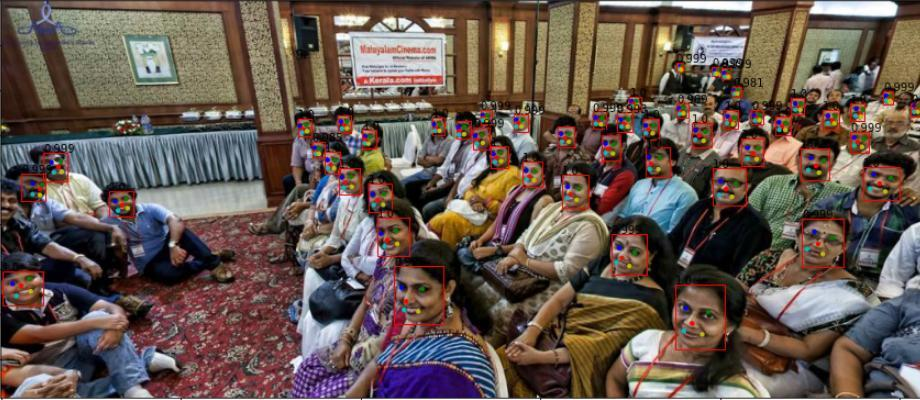
\includegraphics[width=\linewidth]{images/good1.jpg}
        \caption{Модель смогла найти 50 лиц из 61 указанного в ответе.}
    \end{subfigure}

    \centering
    \begin{subfigure}[b]{1.02\linewidth}
        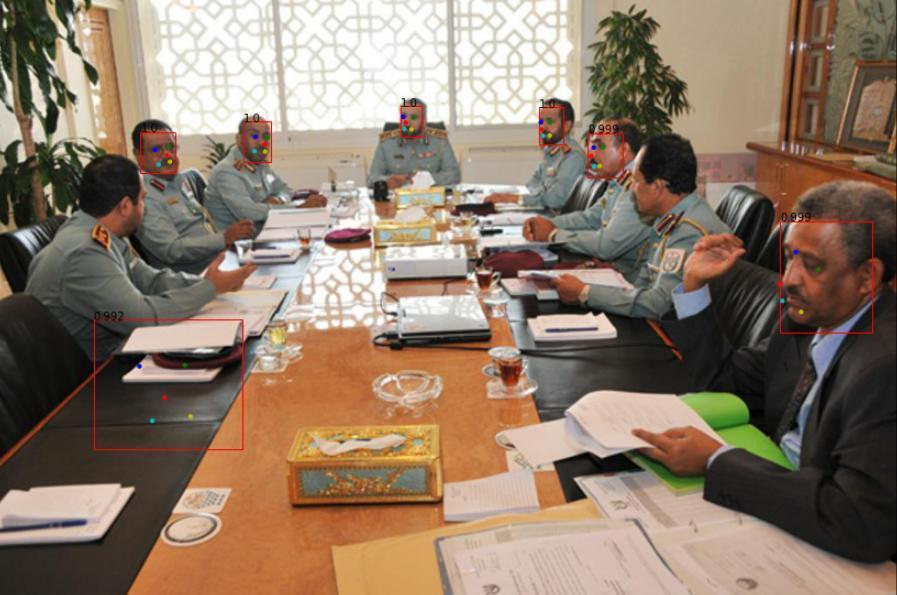
\includegraphics[width=\linewidth]{images/norm1.jpg}
        \caption{Модель хорошо справилась со своей задачей, найдя все повернутые к камере лица, однако она также выделила пустую часть стола.}
    \end{subfigure}
\end{figure}
